\begin{section}{Inplementation}
  \label{sec:simulation}
  We use the \textsc{CUBEP$^3$M} code \cite{bib:Harnois2013} to run
  136 simulations with a box size of 300 Mpc/h and $512^3$ particles.
  The initial conditions are computed using the transfer function
  given by CAMB \cite{bib:Lewis2000} and then propagating the power
  back to $z=100$ with a linear growth factor.  The Zel'dovich
  approximation is used to calculate the displacement and velocity
  fields of the particles.  For these simulations, we use cosmological
  parameters $\Omega_M=0.32$, $\Omega_{\Lambda}=0.679$, $h=0.67$,
  $\sigma_8=0.83$, and $n_s=0.96$.  Different random seeds are used to
  produce the initial conditions for different simulations so that
  they are independent of each other.

  We use Cloud-In-Cell interpolation to estimate the density field
  from the particles.  We then apply the MM reconstruction to these
  fields with a resolution of $128^3$ cells.  A 2D projection of the
  deformed grids and the original density field are given in
  Fig.\ref{fig:simandrec}.  As expected, there is no grid crossing
  after reconstruction.


\begin{figure*}[t!]
  \centering
  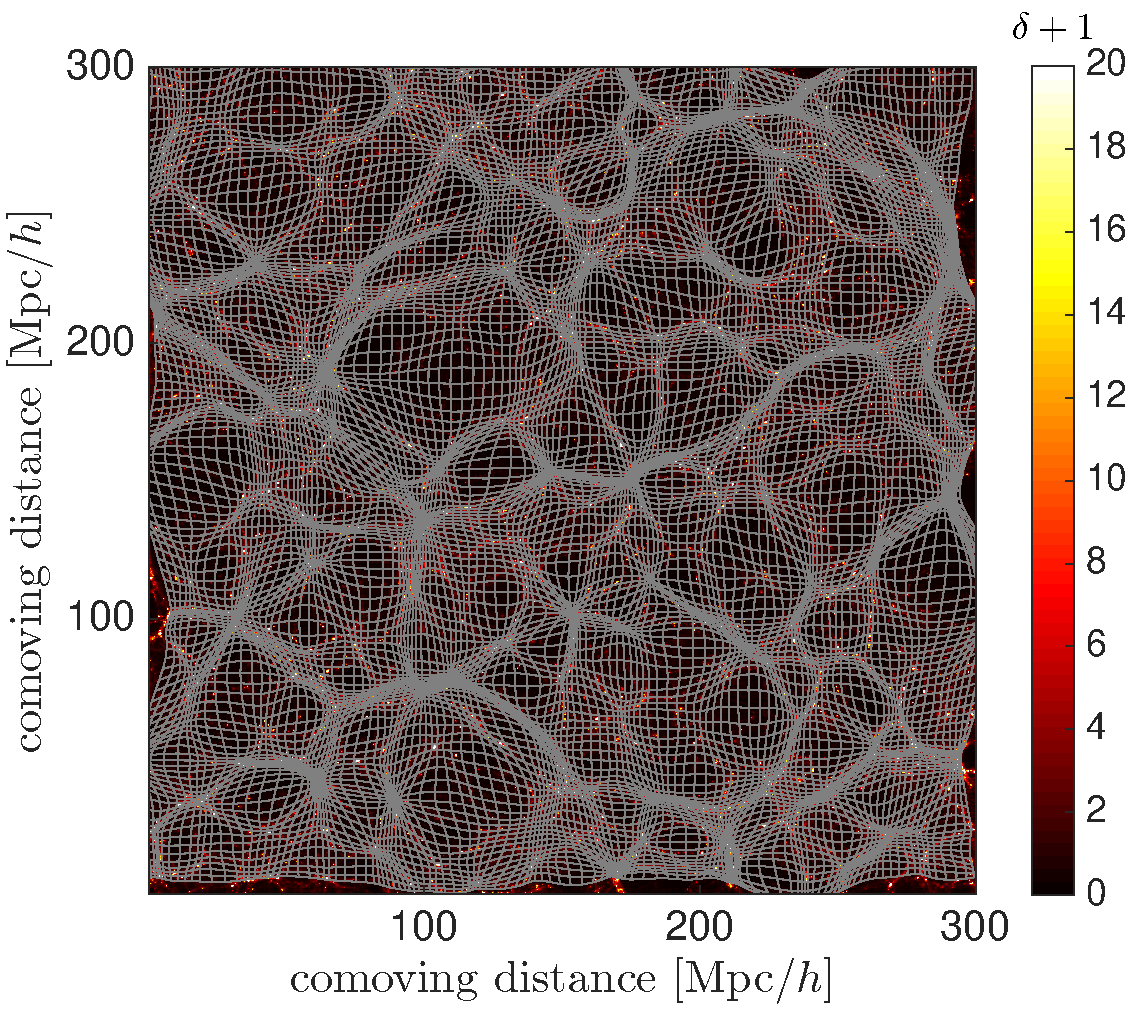
\includegraphics[width=0.9\textwidth]{fig1.pdf}
  \caption{ The 2-D projection of the deformed grid of a sample
    $N$-body simulations is shown as curved white lines. The
    $\delta+1$ field on the deformed grid is shown underneath.}
 \label{fig:simandrec}
\end{figure*}

\end{section}

